\chapter{Diagrammes binaires liquide--vapeur et distillation}\label{ch:b2:liquid-vapour-diagrams}

Un alambic de cuivre transforme un vin à quelques pour cent d'alcool en une eau-de-vie
plusieurs fois plus forte~; une colonne de raffinerie sépare le pétrole brut en ses coupes, du gaz
au fioul lourd. Toutes deux reposent sur un même fait~: la vapeur au-dessus d'un mélange en ébullition est
plus riche que le liquide en constituant le plus volatil. Qu'on répète
l'évaporation et la condensation assez de fois, et la séparation devient aussi
nette qu'on le souhaite --- à une exception près~: aucune distillation, si longue que soit la
colonne, ne porte l'éthanol au-delà d'environ 95 pour cent en masse. Ce chapitre trace
les diagrammes qui décrivent l'ébullition d'un mélange de deux liquides, et s'en sert pour
concevoir une colonne et voir où elle doit s'arrêter.

\begin{recall}
\Cref{ch:b2:chemical-potential}~: le \omterm{def:b2:chemical-potential:chemical-potential}{potentiel chimique}, la \omterm{thm:b2:chemical-potential:raoult}{loi de Raoult} et le
\omterm{def:b2:chemical-potential:ideal-mixture}{mélange idéal}, les \omterm{def:b2:chemical-potential:activity-coefficient}{coefficients d'activité} et les écarts à la \omterm{thm:b2:chemical-potential:raoult}{loi de Raoult}, la
relation de Gibbs--Duhem. \Cref{ch:b2:equilibrium-shifts}~: la \omterm{def:b2:equilibrium-shifts:variance}{variance}. Le
volume de première année, sur les techniques de laboratoire~: distillation simple, liquides miscibles et
non miscibles. Le volume scolaire~: distillation et hydrodistillation.
\end{recall}

\begin{omfigure}
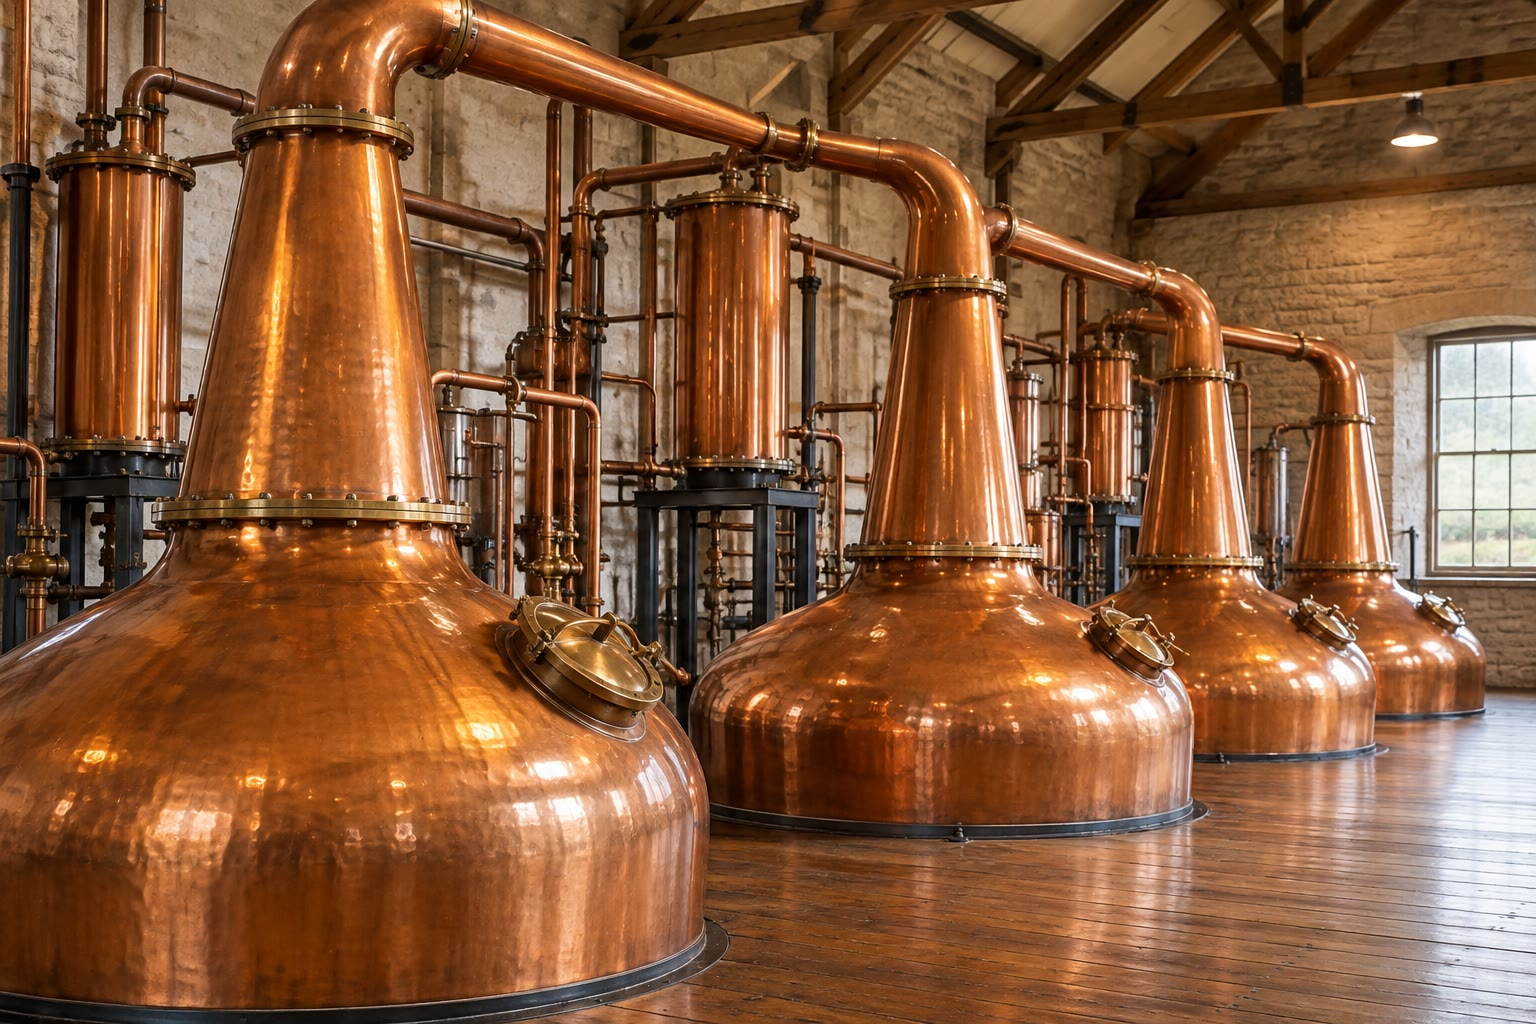
\includegraphics[width=0.62\linewidth]{images/book3/ai/b2-07-pot-stills.jpg}

{\small Alambics de cuivre dans une distillerie. Chaque charge de moût fermenté est
portée à ébullition et sa vapeur condensée~: le premier distillat est plusieurs fois plus riche
en éthanol que le moût, et une seconde distillation le concentre davantage.}
\end{omfigure}

\section{Mélanges idéaux}

Dans ce chapitre, les deux liquides sont numérotés 1 (le plus volatil, de plus basse
température d'ébullition) et 2~; $x$ est la fraction molaire de 1 dans le liquide, $y$ sa
fraction molaire dans la vapeur, traitée comme un gaz parfait.

\begin{definition}[Diagramme binaire]\label{def:b2:liquid-vapour-diagrams:binary-diagram}
Un \emph{diagramme binaire}\index{diagramme binaire} indique, pour un mélange de deux
constituants, quelles phases sont présentes et avec quelles compositions, en
fonction de la composition globale et d'une autre variable. Un
\emph{diagramme isobare}\index{diagramme isobare} se trace dans le plan
(composition, température) à pression fixée~; un \emph{diagramme
isotherme}\index{diagramme isotherme} dans le plan (composition, pression) à
température fixée.
\end{definition}

\begin{definition}[Courbes d'ébullition et de rosée]\label{def:b2:liquid-vapour-diagrams:bubble-dew}
Sur un diagramme liquide--vapeur, la \emph{courbe d'ébullition}\index{courbe d'ebullition@courbe d'ébullition} donne
la composition du liquide en équilibre avec la vapeur, la \emph{courbe de
rosée}\index{courbe de rosee@courbe de rosée} celle de la vapeur en équilibre avec le liquide. Pour un
mélange de composition donnée à pression fixée, le \emph{point de
bulle}\index{point de bulle} est la température à laquelle apparaît la première bulle de
vapeur au chauffage, le \emph{point de rosée}\index{point de rosee@point de rosée} la
température à laquelle apparaît la première goutte de liquide quand on refroidit la vapeur.
\end{definition}

\begin{proposition}[Courbes idéales]\label{prop:b2:liquid-vapour-diagrams:ideal-curves}
Pour un \omterm{def:b2:chemical-potential:ideal-mixture}{mélange idéal} à la température $T$, $p_1^*$ et $p_2^*$ désignant les pressions
de vapeur des liquides purs, la \omterm{def:b2:liquid-vapour-diagrams:bubble-dew}{courbe d'ébullition} du \omterm{def:b2:liquid-vapour-diagrams:binary-diagram}{diagramme isotherme} est
la droite $p = p_2^* + x(p_1^* - p_2^*)$, et la \omterm{def:b2:liquid-vapour-diagrams:bubble-dew}{courbe de rosée} est
l'hyperbole
\[
  p = \frac{1}{y/p_1^* + (1 - y)/p_2^*} .
\]
\end{proposition}

\begin{proof}
La \omterm{thm:b2:chemical-potential:raoult}{loi de Raoult} donne les pressions partielles $p_1 = xp_1^*$ et $p_2 = (1 -
x)p_2^*$~; leur somme est la pression totale, affine en $x$. Dans la vapeur,
$y = p_1/p$, donc $x = yp/p_1^*$ et $1 - x = (1 - y)p/p_2^*$~; par addition,
$1 = p\,[y/p_1^* + (1 - y)/p_2^*]$.
\end{proof}

\begin{proposition}[La vapeur est plus riche en constituant le plus volatil]\label{prop:b2:liquid-vapour-diagrams:richer}
Pour un \omterm{def:b2:chemical-potential:ideal-mixture}{mélange idéal} avec $p_1^* > p_2^*$ et $0 < x < 1$, $y > x$.
\end{proposition}

\begin{proof}
$y = xp_1^*/p$ avec $p = xp_1^* + (1 - x)p_2^* < p_1^*$, puisque $p$ est une
moyenne pondérée de $p_1^*$ et $p_2^*$, strictement comprise entre elles. Donc $y >
x$.
\end{proof}

Le \omterm{def:b2:liquid-vapour-diagrams:binary-diagram}{diagramme isobare} est celui qui décrit une distillation, conduite à la
pression atmosphérique. Il n'a pas de formule simple~: pour chaque température comprise entre
les deux températures d'ébullition, on calcule $p_1^*(T)$ et $p_2^*(T)$ (ici avec
l'équation d'Antoine, $\log_{10}(p^*/\unit{bar}) = A - B/(T + C)$, ajustée sur des
pressions de vapeur mesurées), puis les compositions du liquide et de la vapeur qui
donnent une pression totale de \qty{1.013}{bar}~:
\[
  x = \frac{p - p_2^*(T)}{p_1^*(T) - p_2^*(T)}, \qquad y = \frac{x\,p_1^*(T)}{p} .
\]
La \omterm{def:b2:liquid-vapour-diagrams:bubble-dew}{courbe d'ébullition} n'est plus une droite~; la \omterm{def:b2:liquid-vapour-diagrams:bubble-dew}{courbe de rosée} reste au-dessus d'elle,
la vapeur étant toujours plus riche en constituant léger.

\begin{example}[Benzène et toluène à \qty{90}{\degreeCelsius}]\label{ex:b2:liquid-vapour-diagrams:benzene-toluene}
Le benzène et le toluène forment un mélange presque idéal. À \qty{90}{\degreeCelsius},
les équations d'Antoine donnent $p_1^* = \qty{1.361}{bar}$ (benzène) et $p_2^* =
\qty{0.542}{bar}$ (toluène). Sous \qty{1.013}{bar}~: $x = (1.013 - 0.542)/(1.361 -
0.542) = 0.575$ et $y = 0.575 \times 1.361/1.013 = 0.773$. Un liquide à 57.5~\%
de benzène (en moles) bout à \qty{90}{\degreeCelsius} et donne une vapeur à
77~\%.
% ledger: antoine:benzene.A, antoine:benzene.B, antoine:benzene.C, antoine:toluene.A, antoine:toluene.B, antoine:toluene.C
\end{example}

\begin{omfigure}
\begin{tikzpicture}
\begin{axis}[omphase, width=0.47\linewidth, height=6cm, ymin=78, ymax=113,
  xlabel={$x$, $y$ (benzène)}, ylabel={$T$ (\unit{\degreeCelsius})},
  title={\small isobare, \qty{1.013}{bar}}]
\addplot[omliquidus] table[x=x, y=T] {figdata/out/bachelor-2-liquid-vapour-a.dat};
\addplot[omsolidus] table[x=y, y=T] {figdata/out/bachelor-2-liquid-vapour-a.dat};
\draw[tieline] (axis cs:0.405,95) -- (axis cs:0.626,95);
\fill (axis cs:0.5,95) circle (1.3pt);
\draw[->, thick] (axis cs:0.5,82) -- (axis cs:0.5,104) node[above, font=\scriptsize] {chauffage};
\node[font=\scriptsize] at (axis cs:0.2,85) {liquide};
\node[font=\scriptsize] at (axis cs:0.85,108) {vapeur};
\node[font=\scriptsize, omDef, anchor=north] at (axis cs:0.22,96) {ébullition};
\node[font=\scriptsize, omThm, anchor=south west] at (axis cs:0.62,101) {rosée};
\end{axis}
\end{tikzpicture}\hfill
\begin{tikzpicture}
\begin{axis}[omphase, width=0.47\linewidth, height=6cm, ymin=0.3, ymax=1.1,
  xlabel={$x$, $y$ (benzène)}, ylabel={$p$ (\unit{bar})},
  title={\small isotherme, \qty{80}{\degreeCelsius}}]
\addplot[omliquidus] table[x=x, y=pbub] {figdata/out/bachelor-2-liquid-vapour-b.dat};
\addplot[omsolidus] table[x=x, y=pdew] {figdata/out/bachelor-2-liquid-vapour-b.dat};
\node[font=\scriptsize] at (axis cs:0.75,0.98) {liquide};
\node[font=\scriptsize] at (axis cs:0.2,0.36) {vapeur};
\end{axis}
\end{tikzpicture}

{\small Benzène--toluène, calculé à partir de la \omterm{thm:b2:chemical-potential:raoult}{loi de Raoult} et des équations
d'Antoine. À gauche, sous la pression atmosphérique~: \omterm{def:b2:liquid-vapour-diagrams:bubble-dew}{courbe d'ébullition} (en bleu) et \omterm{def:b2:liquid-vapour-diagrams:bubble-dew}{courbe de rosée}
(en rouge)~; le liquide de composition 0.5 commence à bouillir à
\qty{92.1}{\degreeCelsius} et est entièrement vaporisé à \qty{98.8}{\degreeCelsius}~; à
\qty{95}{\degreeCelsius} (conodale en tirets), il se partage en un liquide de 0.405
et une vapeur de 0.626. À droite, à \qty{80}{\degreeCelsius}~: la \omterm{def:b2:liquid-vapour-diagrams:bubble-dew}{courbe d'ébullition} est
une droite, la \omterm{def:b2:liquid-vapour-diagrams:bubble-dew}{courbe de rosée} une hyperbole, le liquide étant cette fois en haut.}
% ledger: antoine:benzene.A, antoine:toluene.A (all six parameters in figdata/bachelor-2/liquid-vapour.py)
\end{omfigure}

\section{Lire un diagramme}

\begin{proposition}[Variance d'un binaire diphasé]\label{prop:b2:liquid-vapour-diagrams:variance}
Un mélange de deux constituants en deux phases a pour \omterm{def:b2:equilibrium-shifts:variance}{variance} 2. À pression fixée,
la température fixe à elle seule les compositions des deux phases~: on les lit
aux extrémités du segment horizontal qui passe par le point représentatif,
appelé conodale.
\end{proposition}

\begin{proof}
Variables intensives~: $T$, $p$, $x$, $y$. Relations~: égalité des \omterm{def:b2:chemical-potential:chemical-potential}{potentiels
chimiques} de 1 et de 2 entre les phases. $v = 4 - 2 = 2$ (la règle des phases
$v = n - r + 2 - \varphi$ donne le même résultat avec $n = 2$, $r = 0$, $\varphi = 2$).
Fixer $p$ laisse un degré de liberté~: $x(T)$ et $y(T)$ sont les deux courbes.
\end{proof}

\begin{theorem}[Règle des moments]\label{thm:b2:liquid-vapour-diagrams:lever}
Un mélange de composition globale $z$, partagé en un liquide de composition $x$
et une vapeur de composition $y$, contient des quantités $n_L$ de liquide et $n_V$ de
vapeur telles que
\[
  n_L\,(z - x) = n_V\,(y - z), \qquad \frac{n_V}{n_L + n_V} = \frac{z - x}{y - x} .
\]
C'est la \emph{règle des moments}\index{regle des moments@règle des moments}~: chaque phase est d'autant plus
abondante que sa composition est proche de la composition globale, comme les masses sur
un levier qui pivote en $z$.
\end{theorem}

\begin{proof}
Conservation du constituant 1~: $(n_L + n_V)z = n_Lx + n_Vy$, donc $n_L(z - x) =
n_V(y - z)$~; diviser par $n_L + n_V$ et réarranger.
\end{proof}

La \omterm{thm:b2:liquid-vapour-diagrams:lever}{règle des moments} s'applique avec des fractions molaires et des quantités, comme ici, ou avec des
fractions massiques et des masses~: la conservation utilisée est la même.

\begin{method}[Lire un diagramme binaire]\label{met:b2:liquid-vapour-diagrams:read-diagram}
\begin{enumerate}
  \item Placer le point (composition globale, température) et nommer son
        domaine~: liquide, vapeur, ou liquide + vapeur.
  \item Dans un domaine diphasé, tracer la conodale qui passe par le point~; ses extrémités
        donnent les compositions du liquide (sur la \omterm{def:b2:liquid-vapour-diagrams:bubble-dew}{courbe d'ébullition}) et de la
        vapeur (sur la \omterm{def:b2:liquid-vapour-diagrams:bubble-dew}{courbe de rosée}).
  \item Obtenir les proportions des phases par la \omterm{thm:b2:liquid-vapour-diagrams:lever}{règle des moments}.
  \item Pour suivre un chauffage, déplacer le point vers le haut~: la première bulle apparaît
        sur la \omterm{def:b2:liquid-vapour-diagrams:bubble-dew}{courbe d'ébullition}, la dernière goutte disparaît sur la \omterm{def:b2:liquid-vapour-diagrams:bubble-dew}{courbe de rosée}~;
        entre les deux, le liquide s'appauvrit en constituant léger.
\end{enumerate}
\end{method}

\begin{example}[Une vaporisation partielle à \qty{95}{\degreeCelsius}]\label{ex:b2:liquid-vapour-diagrams:flash}
On porte \qty{100}{mol} d'un mélange équimolaire benzène--toluène à
\qty{95}{\degreeCelsius} sous la pression atmosphérique. La conodale donne $x =
0.405$, $y = 0.626$~; la fraction vaporisée vaut $(0.500 - 0.405)/(0.626 - 0.405) =
0.43$~: \qty{43}{mol} de vapeur contenant $43 \times 0.626 = \qty{27}{mol}$ de
benzène, \qty{57}{mol} de liquide en contenant \qty{23}{mol}. Un étage d'équilibre
enrichit, mais seulement un peu.
\end{example}

\section{Mélanges réels et azéotropes}

Lorsque les \omterm{def:b2:chemical-potential:activity-coefficient}{coefficients d'activité} diffèrent de 1 (\cref{ch:b2:chemical-potential}),
les pressions partielles s'écartent des droites de Raoult. Avec un écart
positif ($\gamma > 1$~: les molécules différentes s'attirent moins que les molécules
identiques), la pression totale se situe au-dessus de la droite idéale~; avec un écart négatif,
au-dessous. Si l'écart est assez fort, la pression totale passe par un
extremum.

\begin{definition}[Azéotrope]\label{def:b2:liquid-vapour-diagrams:azeotrope}
Un \emph{azéotrope}\index{azeotrope@azéotrope} est un mélange liquide qui bout sans
changer de composition~: la vapeur qu'il donne a sa propre composition. Un
\emph{azéotrope positif}\index{azeotrope positif@azéotrope positif} (écart positif) présente
un maximum de pression sur le \omterm{def:b2:liquid-vapour-diagrams:binary-diagram}{diagramme isotherme} et un minimum de température
d'ébullition sur le \omterm{def:b2:liquid-vapour-diagrams:binary-diagram}{diagramme isobare}~; un \emph{azéotrope négatif}\index{azeotrope negatif@azéotrope négatif}
présente l'inverse.
\end{definition}

\begin{theorem}[Gibbs--Konovalov]\label{thm:b2:liquid-vapour-diagrams:konovalov}
Sur un \omterm{def:b2:liquid-vapour-diagrams:binary-diagram}{diagramme binaire} liquide--vapeur, en un extremum de la pression totale (à
température fixée) ou de la température d'ébullition (à pression fixée), le
liquide et la vapeur ont la même composition. Réciproquement, là où les
deux compositions sont égales, les courbes ont une tangente horizontale commune.
\end{theorem}

\begin{proof}[Démonstration à température fixée]
La relation de Gibbs--Duhem pour le liquide à $T$ fixée (le faible effet de $p$
sur le liquide étant négligé) s'écrit $x\,d\mu_1 + (1 - x)\,d\mu_2 = 0$. À l'équilibre,
$\mu_i = \mu_i^\circ + RT\ln(p_i/p^\circ)$ avec $p_1 = yp$, $p_2 = (1 - y)p$, donc
\[
  x\,d\ln(yp) + (1 - x)\,d\ln((1 - y)p) = 0
  \quad\Longrightarrow\quad
  d\ln p = -\Big(\frac{x}{y} - \frac{1 - x}{1 - y}\Big)dy
  = \frac{y - x}{y(1 - y)}\,dy .
\]
Comme $y$ croît avec $x$ (sinon le liquide serait instable),
$dp/dx = 0$ exactement là où $y = x$. Le cas isobare découle d'un
calcul analogue qui conserve la dépendance en température des $\mu_i^\circ$~; il n'est
pas mené ici.
\end{proof}

La formule en dit davantage~: là où $y > x$, la pression croît avec $x$ ---
ajouter le constituant qui s'enrichit dans la vapeur rend le liquide plus
volatil, ce qui est la première loi de Konovalov.

\begin{example}[Éthanol et eau]\label{ex:b2:liquid-vapour-diagrams:ethanol-water}
L'éthanol et l'eau s'écartent positivement de la \omterm{thm:b2:chemical-potential:raoult}{loi de Raoult} et forment un \omterm{def:b2:liquid-vapour-diagrams:azeotrope}{azéotrope}
à 95~\% d'éthanol en masse sous la pression atmosphérique. Avec $M = 46.07$ et
\qty{18.02}{g/mol}, sa fraction molaire en éthanol vaut
\[
  x_{\text{az}} = \frac{95/46.07}{95/46.07 + 5/18.02} = 0.881 .
\]
Il bout un peu au-dessous de l'éthanol pur (\qty{78.3}{\degreeCelsius}). Le diagramme
ci-dessous est calculé à partir d'un modèle d'activité à un paramètre, $\ln\gamma_1 = A(1 -
x)^2$, $\ln\gamma_2 = Ax^2$, dont le paramètre ($A = 1.09$) est ajusté pour que
l'\omterm{def:b2:liquid-vapour-diagrams:azeotrope}{azéotrope} tombe à cette composition~: le modèle reproduit l'allure, et
place l'\omterm{def:b2:liquid-vapour-diagrams:azeotrope}{azéotrope} à \qty{77.9}{\degreeCelsius}.
% ledger: azeo:ethanol-water.w, aw:C, aw:H, aw:O, antoine:ethanol.A, antoine:ethanol.B, antoine:ethanol.C, antoine:water.A, antoine:water.B, antoine:water.C
\end{example}

\begin{omfigure}
\begin{tikzpicture}
\begin{axis}[omphase, width=0.47\linewidth, height=6cm, ymin=76, ymax=101,
  xlabel={$x$, $y$ (éthanol)}, ylabel={$T$ (\unit{\degreeCelsius})},
  title={\small éthanol--eau (modèle)}]
\addplot[omliquidus] table[x=x, y=T] {figdata/out/bachelor-2-liquid-vapour-c.dat};
\addplot[omsolidus] table[x=y, y=T] {figdata/out/bachelor-2-liquid-vapour-c.dat};
\fill (axis cs:0.881,77.92) circle (1.5pt);
\draw[densely dotted] (axis cs:0.881,77.92) -- (axis cs:0.881,76);
\node[font=\scriptsize, anchor=south] at (axis cs:0.80,80.5) {azéotrope};
\draw[thin] (axis cs:0.80,80.5) -- (axis cs:0.875,78.2);
\node[font=\scriptsize] at (axis cs:0.25,79.5) {liquide};
\node[font=\scriptsize] at (axis cs:0.5,95) {vapeur};
\end{axis}
\end{tikzpicture}\hfill
\begin{tikzpicture}
\begin{axis}[omphase, width=0.47\linewidth, height=6cm, ymin=78, ymax=120,
  xlabel={$x$, $y$ (constituant 1)}, ylabel={$T$ (\unit{\degreeCelsius})},
  title={\small écart négatif (modèle)}]
\addplot[omliquidus] table[x=x, y=T] {figdata/out/bachelor-2-liquid-vapour-d.dat};
\addplot[omsolidus] table[x=y, y=T] {figdata/out/bachelor-2-liquid-vapour-d.dat};
\fill (axis cs:0.29,116.7) circle (1.5pt);
\node[font=\scriptsize, anchor=west] at (axis cs:0.33,118) {azéotrope};
\node[font=\scriptsize] at (axis cs:0.6,85) {liquide};
\node[font=\scriptsize] at (axis cs:0.75,116) {vapeur};
\end{axis}
\end{tikzpicture}

{\small À gauche~: éthanol--eau sous la pression atmosphérique, d'après un modèle à un paramètre
ajusté sur la composition de l'\omterm{def:b2:liquid-vapour-diagrams:azeotrope}{azéotrope} (0.881)~; l'\omterm{def:b2:liquid-vapour-diagrams:azeotrope}{azéotrope} bout au-dessous des
deux liquides purs. À droite~: un couple modèle à fort écart négatif
($A = -2.0$, pressions de vapeur du benzène et du toluène)~; l'\omterm{def:b2:liquid-vapour-diagrams:azeotrope}{azéotrope} bout
au-dessus des deux.}
% ledger: azeo:ethanol-water.w, antoine:ethanol.A, antoine:water.A (model in figdata/bachelor-2/liquid-vapour.py)
\end{omfigure}

\section{La distillation fractionnée}

\begin{definition}[Distillation fractionnée]\label{def:b2:liquid-vapour-diagrams:fractional-distillation}
La \emph{distillation fractionnée}\index{distillation fractionnee@distillation fractionnée} sépare les
constituants d'un mélange liquide dans une colonne où une vapeur ascendante et un
liquide descendant sont mis en contact de façon répétée. Un \emph{plateau
théorique}\index{plateau theorique@plateau théorique} est un étage de la colonne dont la vapeur et le
liquide sortants sont en équilibre l'un avec l'autre. Le \emph{taux de
reflux}\index{taux de reflux} est le rapport de la quantité de condensat renvoyée
en tête de colonne à la quantité soutirée comme distillat.
\end{definition}

Sur chaque plateau, la vapeur venue d'en dessous barbote dans le liquide venu d'en haut~; elle
en ressort enrichie en constituant léger, le liquide appauvri. En tête, la vapeur
est condensée, une partie renvoyée en reflux, le reste soutiré comme
distillat~; au pied, un bouilleur vaporise une partie du liquide. À
\textit{reflux total}, rien n'est soutiré~: la colonne fonctionne alors au mieux,
et la vapeur qui quitte un plateau a la composition du liquide qui descend
sur lui.


Pour un couple idéal, la \textit{volatilité relative} $\alpha = p_1^*/p_2^*$
varie peu le long de la colonne~: de 2.60 à la température d'ébullition du benzène à
2.35 à celle du toluène. Sur chaque \omterm{def:b2:liquid-vapour-diagrams:fractional-distillation}{plateau théorique},
\[
  \frac{y}{1 - y} = \frac{xp_1^*}{(1 - x)p_2^*} = \alpha\,\frac{x}{1 - x} .
\]

\begin{omfigure}
\begin{minipage}[b]{0.58\linewidth}\centering
\begin{tikzpicture}[font=\small, >={Stealth}, scale=0.8, every node/.style={transform shape}]
  \draw[thick, fill=gray!8] (0,0) rectangle (1.8,7);
  \foreach \k in {1,...,6} {
    \pgfmathsetmacro{\yy}{\k}
    \ifodd\k
      \draw[thick] (0,\yy) -- (1.45,\yy); \draw[thick] (1.45,\yy) -- (1.45,\yy-0.55);
    \else
      \draw[thick] (0.35,\yy) -- (1.8,\yy); \draw[thick] (0.35,\yy) -- (0.35,\yy-0.55);
    \fi
    \fill[omDef!25] (0.02,\yy) rectangle (1.78,\yy+0.12);
  }
  \foreach \k in {1,...,6} \node[font=\scriptsize, anchor=east] at (-0.1,\k) {plateau \k};
  \draw[->, thick, omThm] (0.9,7.0) -- (0.9,7.9) -- (2.8,7.9);
  \draw[thick, fill=white] (2.8,7.6) rectangle (3.6,8.2);
  \node[anchor=west, font=\scriptsize] at (3.65,7.9) {condenseur};
  \draw[->, thick, omDef] (3.2,7.6) -- (3.2,5.6);
  \draw[thick, fill=omDef!20] (2.7,5.0) rectangle (3.7,5.6);
  \node[font=\scriptsize, anchor=west] at (3.75,5.3) {ballon de reflux};
  \draw[->, thick, omDef] (2.7,5.3) -- (2.1,5.3) -- (2.1,6.6) -- (1.8,6.6);
  \node[font=\scriptsize, anchor=west, omDef] at (2.15,6.1) {reflux};
  \draw[->, thick, omDef] (3.2,5.0) -- (3.2,4.4) -- (4.4,4.4) node[right] {distillat};
  \draw[->, thick] (-2.2,3.5) -- (0,3.5) node[pos=0, left] {alimentation};
  \draw[thick, fill=omDef!20] (0.2,-1.3) rectangle (1.6,-0.6);
  \node[font=\scriptsize] at (0.9,-0.95) {bouilleur};
  \draw[thick, omDef] (0.9,0) -- (0.9,-0.6);
  \draw[->, thick, omThm] (1.6,-0.8) -- (2.1,-0.8) -- (2.1,0.4) -- (1.8,0.4);
  \draw[->, thick, omDef] (0.9,-1.3) -- (0.9,-1.8) -- (2.6,-1.8) node[right] {résidu};
  \draw[->, omThm, thick] (2.6,1.5) -- (2.6,3.0) node[midway, right, font=\scriptsize, align=left] {la vapeur\\ monte};
  \draw[->, omDef, thick] (-1.4,5.8) -- (-1.4,4.3) node[midway, left, font=\scriptsize, align=right] {le liquide\\ descend};
\end{tikzpicture}
\end{minipage}\hfill
\begin{minipage}[b]{0.34\linewidth}\centering
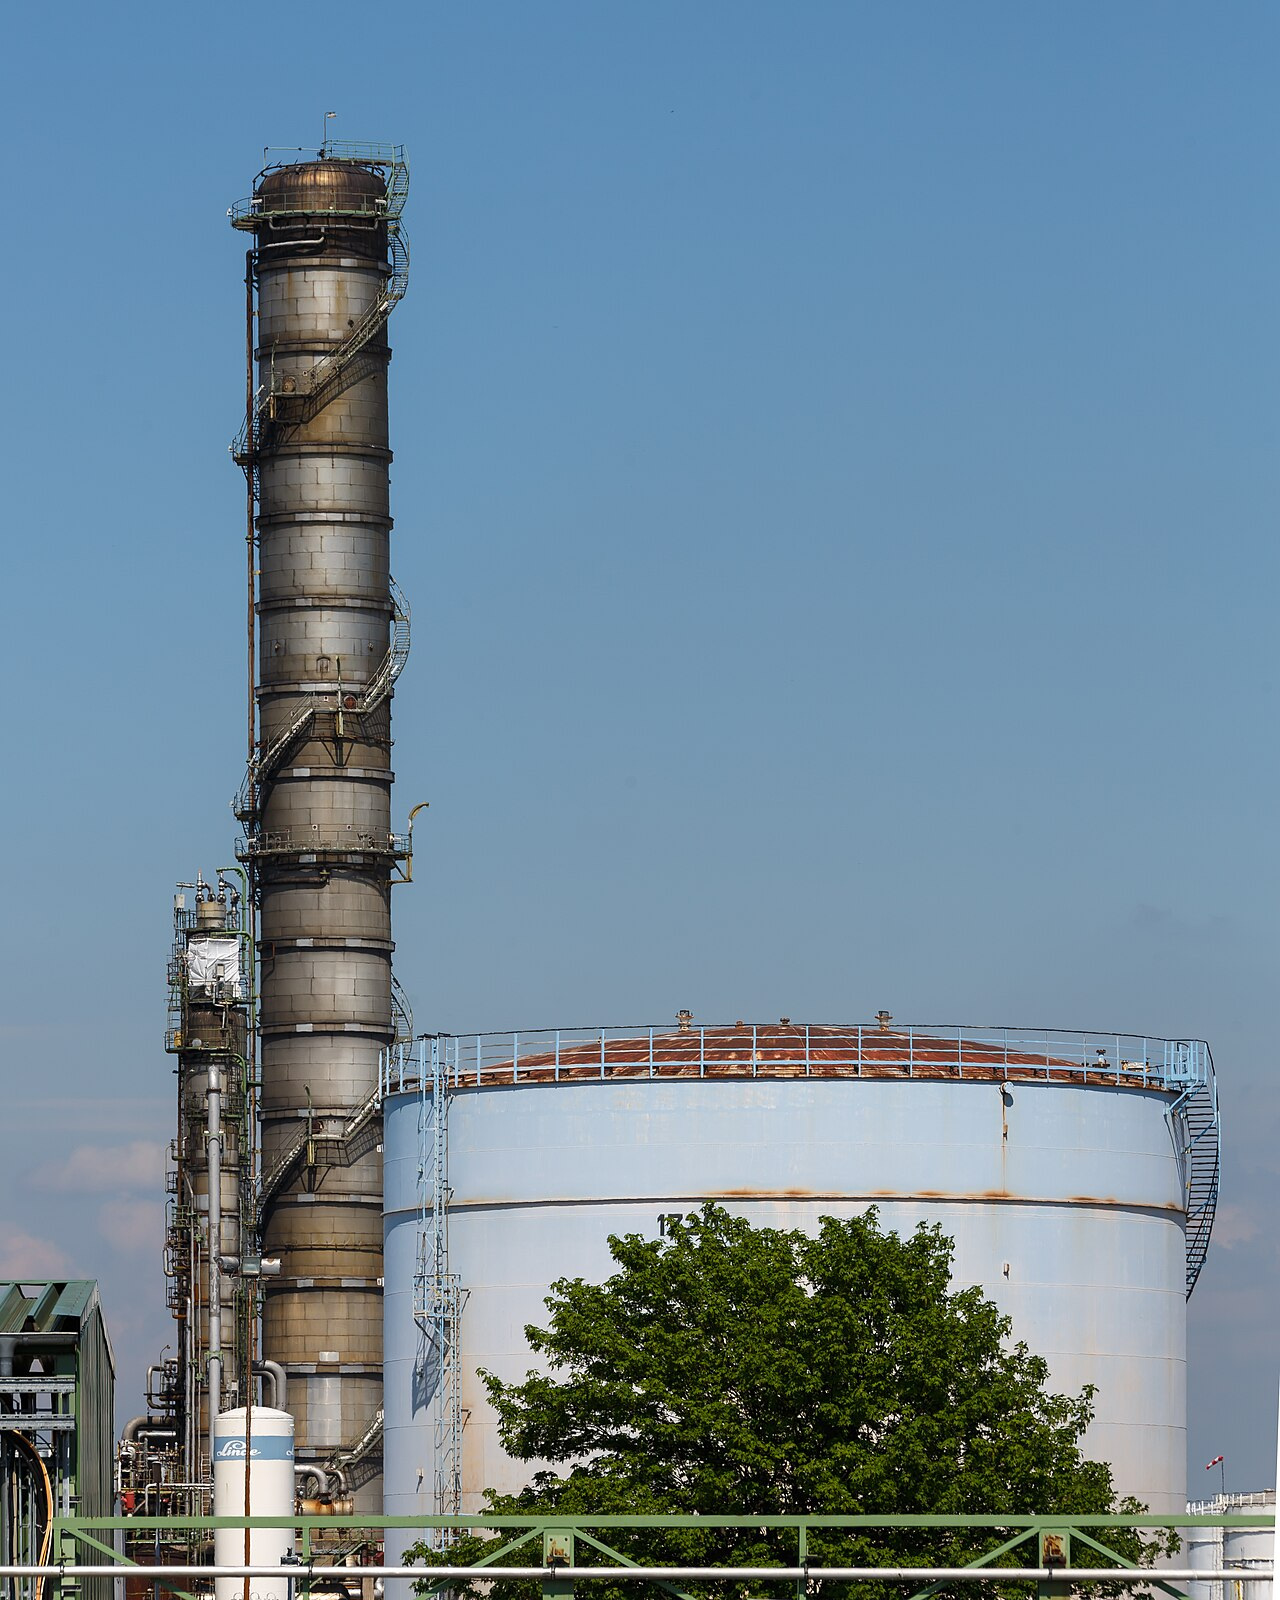
\includegraphics[width=\linewidth]{images/book3/refinery-column.jpg}
\end{minipage}

{\small À gauche~: une colonne à plateaux. Le liquide traverse chaque plateau et descend par
le trop-plein vers le plateau inférieur~; la vapeur monte à travers les plateaux et barbote
dans le liquide. La vapeur condensée est en partie renvoyée en reflux~; le
bouilleur, au pied, fournit la vapeur. À droite~: une colonne de distillation d'une
raffinerie (Cologne, 2014), qui compte des dizaines de plateaux. (Photographie~: CEphoto,
Uwe Aranas, CC BY-SA 3.0, Wikimedia Commons.)}
\end{omfigure}

\begin{proposition}[Fenske]\label{prop:b2:liquid-vapour-diagrams:fenske}
À reflux total, avec une volatilité relative $\alpha$ constante, le nombre de
\omterm{def:b2:liquid-vapour-diagrams:fractional-distillation}{plateaux théoriques} nécessaires pour passer d'un liquide de pied $x_B$ à un distillat
$x_D$ vaut au moins
\[
  N_{\min} = \frac{1}{\ln\alpha}\,\ln\!\left[\frac{x_D}{1 - x_D}\cdot\frac{1 - x_B}{x_B}\right] .
\]
\end{proposition}

\begin{proof}
Numérotons les plateaux à partir du bas, le bouilleur étant le plateau 1. À reflux total,
le liquide qui descend sur le plateau $k + 1$ a la composition de la vapeur
qui quitte le plateau $k$~: $x_{k+1} = y_k$. Avec $r = x/(1 - x)$, chaque plateau donne
$r(y_k) = \alpha\,r(x_k)$, donc $r(x_{k+1}) = \alpha\,r(x_k)$, et après $N$
plateaux la vapeur condensée vérifie $r(x_D) = \alpha^N r(x_B)$. En prenant les logarithmes,
on obtient $N$. Avec un reflux fini, le liquide qui descend est plus pauvre que la
vapeur qui monte, chaque plateau enrichit moins, et il faut davantage de plateaux.
\end{proof}

Sur le diagramme $(x, y)$, la même construction est un escalier entre la
courbe d'équilibre et la diagonale $y = x$~: chaque marche représente un \omterm{def:b2:liquid-vapour-diagrams:fractional-distillation}{plateau
théorique}.

\begin{omfigure}
\begin{tikzpicture}
\begin{axis}[width=0.55\linewidth, height=0.55\linewidth, xmin=0, xmax=1,
  ymin=0, ymax=1, axis x line=bottom, axis y line=left,
  xlabel={$x$ (benzène, liquide)}, ylabel={$y$ (benzène, vapeur)},
  tick label style={font=\small}, label style={font=\small}]
\addplot[omThm, thick] table[x=x, y=y] {figdata/out/bachelor-2-liquid-vapour-f-eq.dat};
\addplot[black!50] coordinates {(0,0) (1,1)};
\addplot[omDef, thick] table[x=x, y=y] {figdata/out/bachelor-2-liquid-vapour-f.dat};
\draw[densely dotted] (axis cs:0.95,0) -- (axis cs:0.95,0.95);
\draw[densely dotted] (axis cs:0.05,0) -- (axis cs:0.05,0.05);
\node[font=\scriptsize, anchor=south east] at (axis cs:0.945,0.02) {$x_D$};
\node[font=\scriptsize, anchor=south west] at (axis cs:0.05,0.02) {$x_B$};
\end{axis}
\end{tikzpicture}

{\small Plateaux à reflux total pour benzène--toluène, à partir d'un distillat de
0.95~: chaque marche horizontale va d'une vapeur au liquide en
équilibre avec elle (un plateau), chaque marche verticale de ce liquide à la
vapeur du plateau inférieur. Sept marches amènent le liquide au-dessous de $x_B = 0.05$~;
la formule de Fenske donne 6.5.}
% ledger: antoine:benzene.A, antoine:toluene.A (computed in figdata/bachelor-2/liquid-vapour.py)
\end{omfigure}

\begin{proposition}[Une colonne ne franchit pas un azéotrope]\label{prop:b2:liquid-vapour-diagrams:azeotrope-limit}
Pour un mélange présentant un \omterm{def:b2:liquid-vapour-diagrams:azeotrope}{azéotrope}, une colonne alimentée d'un côté de la
composition azéotropique fournit au mieux l'\omterm{def:b2:liquid-vapour-diagrams:azeotrope}{azéotrope} à une extrémité et le constituant pur
de ce côté à l'autre.
\end{proposition}

\begin{proof}
À l'\omterm{def:b2:liquid-vapour-diagrams:azeotrope}{azéotrope}, la courbe d'équilibre rencontre la diagonale~: $y = x$. Au voisinage,
chaque marche de l'escalier devient infiniment petite~: aucun nombre fini de
plateaux ne l'atteint, et aucun ne la franchit.
\end{proof}

\begin{method}[Prévoir une distillation fractionnée]\label{met:b2:liquid-vapour-diagrams:predict-distillation}
\begin{enumerate}
  \item Repérer sur le \omterm{def:b2:liquid-vapour-diagrams:binary-diagram}{diagramme isobare} le point de plus basse température d'ébullition accessible à partir de
        l'alimentation~: un constituant pur ou un \omterm{def:b2:liquid-vapour-diagrams:azeotrope}{azéotrope positif}. Il sort
        en tête.
  \item Le point de plus haute température d'ébullition du même côté (constituant pur ou
        \omterm{def:b2:liquid-vapour-diagrams:azeotrope}{azéotrope négatif}) reste dans le bouilleur.
  \item En présence d'un \omterm{def:b2:liquid-vapour-diagrams:azeotrope}{azéotrope}, regarder de quel côté se trouve l'alimentation~: seul le
        constituant pur de ce côté peut être obtenu.
  \item Pour le nombre de plateaux, utiliser la formule de Fenske ou l'escalier,
        puis ajouter des plateaux pour le reflux fini réellement utilisé.
\end{enumerate}
\end{method}

Pour l'éthanol et l'eau introduits à moins de 0.881, la tête fournit au mieux
l'\omterm{def:b2:liquid-vapour-diagrams:azeotrope}{azéotrope} et le pied de l'eau~: aucune colonne ne donne d'éthanol absolu. Éliminer
le dernier pour cent exige une autre méthode --- un tamis moléculaire qui adsorbe l'eau, ou
un troisième constituant ajouté pour briser l'\omterm{def:b2:liquid-vapour-diagrams:azeotrope}{azéotrope}.

\begin{omfigure}
\begin{tikzpicture}[font=\small, scale=0.95, >={Stealth}]
  \pic[transform shape] at (0,0) {heatingmantle};
  \pic[transform shape] at (0,0) {rbflask={0.45}{orange!25}};
  \foreach \x/\y in {-0.35/0.25,0.05/0.18,0.35/0.3}
    \fill[black!55] (\x,\y) circle (0.06);
  % Vigreux column from the flask neck (0,3) to (0,6)
  \draw[om glass] (-0.22,3.0) -- (-0.22,6.0) (0.22,3.0) -- (0.22,6.0);
  \foreach \yy in {3.4,3.9,4.4,4.9,5.4} {
    \draw[om glass] (-0.22,\yy) -- (-0.06,\yy+0.18) -- (-0.22,\yy+0.3);
    \draw[om glass] (0.22,\yy+0.15) -- (0.06,\yy+0.33) -- (0.22,\yy+0.45);
  }
  \pic[transform shape] (s) at (0,6.0) {stillhead};
  \pic[transform shape] at ($(s-top)+(0,-0.75)$) {thermometer};
  \pic[transform shape, rotate=-20] (c) at (s-arm) {liebig={3.4}};
  % ground-glass joint between the head's side arm and the condenser
  \draw[om glass, fill=white, rotate around={-20:(s-arm)}] ($(s-arm)+(-0.12,-0.17)$) rectangle ($(s-arm)+(0.14,0.17)$);
  \coordinate (cend) at ($(s-arm)+(-20:3.4)$);
  \pic[transform shape] (a) at (cend) {adapter};
  \pic[transform shape] at ($(a-tip)+(0,-2.4)$) {erlenmeyer={0.22}{orange!12}};
  \draw[<-, omProp, thick] (-0.25,4.6) -- (-1.6,4.6) node[left, text=black,
    align=right] {colonne de Vigreux\\ (les indentations multiplient\\ les contacts)};
  \draw[<-, omProp, thick] (0.12,6.72) -- (-1.4,7.4) node[left, text=black,
    align=right] {réservoir du thermomètre\\ au niveau de la tubulure};
  \draw[<-, omProp, thick] (1.08,0.3) -- (2.3,-0.2) node[right, text=black]
    {chauffe-ballon};
  \draw[<-, omProp, thick] ($(a-tip)+(0.75,-2.0)$) -- ++(1.0,0.2)
    node[right, text=black] {distillat};
\end{tikzpicture}

{\small \omterm{def:b2:liquid-vapour-diagrams:fractional-distillation}{Distillation fractionnée} au laboratoire. Une colonne de Vigreux placée entre
le ballon et la tête joue le rôle de quelques \omterm{def:b2:liquid-vapour-diagrams:fractional-distillation}{plateaux théoriques}~: la vapeur
se condense sur ses indentations et se revaporise en montant. La
température en tête reste à la température d'ébullition du constituant le plus volatil
tant qu'il distille, puis s'élève.}
\end{omfigure}

\begin{inthelab}[Séparer deux liquides par distillation fractionnée]
On remplit le ballon à moitié au plus, avec de la pierre ponce, et on chauffe doucement
pour que l'anneau de vapeur qui se condense monte lentement dans la colonne~: une colonne
noyée par un chauffage trop rapide perd ses plateaux. On relève la température en tête tous les
quelques millilitres~; on change de récipient quand elle commence à monter (une
\textit{fraction} est recueillie sur chaque palier de température), et on arrête le chauffage
avant que le ballon soit à sec.
\end{inthelab}

\section{Liquides partiellement miscibles et non miscibles}

\begin{definition}[Lacune de miscibilité]\label{def:b2:liquid-vapour-diagrams:miscibility-gap}
Une \emph{lacune de miscibilité}\index{lacune de miscibilite@lacune de miscibilité} est le domaine de compositions
globales sur lequel deux liquides, à une température donnée, se séparent en deux
phases liquides, chacune saturée de l'autre constituant. Un
\emph{hétéroazéotrope}\index{heteroazeotrope@hétéroazéotrope} est le point d'ébullition d'un tel
liquide à deux phases~: les deux phases liquides et la vapeur coexistent à une
température fixée et avec une composition de vapeur fixée.
\end{definition}

À l'\omterm{def:b2:liquid-vapour-diagrams:miscibility-gap}{hétéroazéotrope}, deux constituants se répartissent en trois phases~: à pression
fixée, la \omterm{def:b2:equilibrium-shifts:variance}{variance} vaut $2 + 2 - 3 - 1 = 0$. La température reste
constante, comme à la température d'ébullition d'un liquide pur, tant que les deux phases liquides
subsistent.

\begin{omfigure}
\begin{tikzpicture}[font=\small, x=6cm, y=0.08cm]
  \draw[->] (0,0) -- (1.05,0) node[right] {$x$};
  \draw[->] (0,0) -- (0,62) node[above] {$T$};
  \node[below] at (0,0) {2}; \node[below] at (1,0) {1};
  % boiling points: 2 at 50, 1 at 42; heteroazeotrope at 25 with layers 0.1 and 0.85, vapour 0.6
  \draw[omliquidus] (0,50) .. controls (0.04,38) and (0.08,30) .. (0.1,25);
  \draw[omliquidus] (1,42) .. controls (0.95,34) and (0.9,28) .. (0.85,25);
  \draw[omsolidus] (0,50) .. controls (0.25,46) and (0.5,35) .. (0.6,25);
  \draw[omsolidus] (1,42) .. controls (0.9,37) and (0.7,30) .. (0.6,25);
  \draw[thick] (0.1,25) -- (0.85,25);
  \draw[omliquidus] (0.1,25) -- (0.07,2);
  \draw[omliquidus] (0.85,25) -- (0.9,2);
  \fill (0.6,25) circle[radius=2pt];
  \node[font=\scriptsize] at (0.47,6) {deux phases liquides};
  \node[font=\scriptsize] at (0.5,55) {vapeur};
  \node[font=\scriptsize] at (0.035,12) {L$_2$};
  \node[font=\scriptsize] at (0.96,12) {L$_1$};
  \node[font=\scriptsize, align=center] at (0.3,33) {L$_2$ + V};
  \node[font=\scriptsize, anchor=west] at (1.06,36) {L$_1$ + V};
  \draw[thin] (1.06,36) -- (0.86,29.5);
  \node[font=\scriptsize, anchor=north] at (0.6,24) {hétéroazéotrope};
\end{tikzpicture}

{\small \omterm{def:b2:liquid-vapour-diagrams:binary-diagram}{Diagramme isobare} schématique de deux liquides partiellement miscibles. Au-dessous de la
température de l'\omterm{def:b2:liquid-vapour-diagrams:miscibility-gap}{hétéroazéotrope}, le liquide se sépare en deux phases L$_1$ et
L$_2$ sur un large domaine de compositions (la \omterm{def:b2:liquid-vapour-diagrams:miscibility-gap}{lacune de miscibilité})~; sur le
palier horizontal, les deux phases bouillent ensemble en donnant une vapeur de
composition fixée (point).}
\end{omfigure}

\begin{definition}[Entraînement à la vapeur]\label{def:b2:liquid-vapour-diagrams:steam-distillation}
L'\emph{entraînement à la vapeur}\index{entrainement a la vapeur@entraînement à la vapeur} est la distillation d'un
liquide non miscible à l'eau, obtenue en y insufflant de la vapeur d'eau~: le mélange bout
au-dessous de la température d'ébullition des deux liquides, et le distillat se sépare en
deux phases.
\end{definition}

L'\omterm{def:b2:liquid-vapour-diagrams:steam-distillation}{entraînement à la vapeur} ne diffère de l'hydrodistillation du volume scolaire
que par la manière d'apporter l'eau~: de la vapeur insufflée à travers la matière, plutôt
que de la matière portée à ébullition dans l'eau. La thermodynamique est la même.

\begin{proposition}[Ébullition de deux liquides non miscibles]\label{prop:b2:liquid-vapour-diagrams:steam}
Deux liquides non miscibles en contact bouillent à la température où la somme de
leurs pressions de vapeur est égale à la pression extérieure, $p_1^*(T) + p_2^*(T) =
p$, inférieure aux deux températures d'ébullition. Le distillat contient les deux liquides
dans le rapport massique
\[
  \frac{m_1}{m_2} = \frac{p_1^*\,M_1}{p_2^*\,M_2} .
\]
\end{proposition}

\begin{proof}
Chaque liquide pur exerce sa propre pression de vapeur, quelle que soit la quantité de
l'autre~: la pression totale au-dessus des deux phases est $p_1^* + p_2^*$, qui
atteint $p$ à une température où chaque $p_i^*$ est inférieure à $p$. Dans la
vapeur, les quantités sont proportionnelles aux pressions partielles, $n_1/n_2 =
p_1^*/p_2^*$~; il reste à multiplier par $M_1/M_2$.
\end{proof}

\begin{omfigure}
\begin{tikzpicture}
\begin{axis}[width=0.6\linewidth, height=5.5cm, xmin=70, xmax=100, ymin=0, ymax=1.6,
  axis x line=bottom, axis y line=left, xlabel={$T$ (\unit{\degreeCelsius})},
  ylabel={$p$ (\unit{bar})}, tick label style={font=\small},
  label style={font=\small}, clip=false]
\addplot[omProp, thick] table[x=t, y=ptol] {figdata/out/bachelor-2-liquid-vapour-e.dat};
\addplot[omDef, thick] table[x=t, y=pwat] {figdata/out/bachelor-2-liquid-vapour-e.dat};
\addplot[black, very thick] table[x=t, y=psum] {figdata/out/bachelor-2-liquid-vapour-e.dat};
\draw[densely dashed] (axis cs:70,1.013) -- (axis cs:100,1.013) node[right, font=\scriptsize] {\qty{1.013}{bar}};
\draw[densely dotted] (axis cs:84.3,0) -- (axis cs:84.3,1.013);
\node[font=\scriptsize, anchor=south east] at (axis cs:84.3,1.05) {\qty{84.3}{\degreeCelsius}};
\node[font=\scriptsize, anchor=west] at (axis cs:96,1.45) {somme};
\node[font=\scriptsize, omDef, anchor=south] at (axis cs:77,0.46) {eau};
\node[font=\scriptsize, omProp, anchor=north west] at (axis cs:88,0.5) {toluène};
\end{axis}
\end{tikzpicture}

{\small Toluène et eau, non miscibles~: pressions de vapeur de chaque liquide et
leur somme. Les deux phases bouillent ensemble à \qty{84.3}{\degreeCelsius}, au-dessous
de l'eau (\qty{100}{\degreeCelsius}) et du toluène (\qty{110.6}{\degreeCelsius})~;
le distillat entraîne 4.1 g de toluène par gramme d'eau.}
% ledger: antoine:toluene.A, antoine:water.A, aw:C, aw:H, aw:O (computed in figdata/bachelor-2/liquid-vapour.py)
\end{omfigure}

Les molécules lourdes et fragiles des essences végétales distillent ainsi à un peu
moins de \qty{100}{\degreeCelsius}, bien au-dessous de leur propre température d'ébullition, avec
peu de décomposition~; le prix à payer est un distillat composé surtout d'eau.

\section{Exercices}

\begin{exercise}[$\star$]\label{exo:b2:liquid-vapour-diagrams:1}
Sur le \omterm{def:b2:liquid-vapour-diagrams:binary-diagram}{diagramme isobare} benzène--toluène, lire les températures d'ébullition des liquides
purs, le \omterm{def:b2:liquid-vapour-diagrams:bubble-dew}{point de bulle} d'un liquide de composition 0.2 et la composition de
sa première vapeur.
\end{exercise}

\begin{exercise}[$\star$]\label{exo:b2:liquid-vapour-diagrams:2}
À \qty{80}{\degreeCelsius}, les pressions de vapeur du benzène et du toluène valent
\qty{1.010}{bar} et \qty{0.388}{bar}. Calculer, pour un liquide équimolaire, la
pression à laquelle il commence à bouillir et la composition de la vapeur.
\end{exercise}

\begin{exercise}[$\star$]\label{exo:b2:liquid-vapour-diagrams:3}
\qty{10}{mol} d'un mélange de composition globale 0.30 se trouvent à une température
où le liquide a pour composition 0.20 et la vapeur 0.45. Calculer les quantités
de chaque phase.
\end{exercise}

\begin{exercise}[$\star$]\label{exo:b2:liquid-vapour-diagrams:4}
Calculer la \omterm{def:b2:equilibrium-shifts:variance}{variance} d'un mélange benzène--toluène (a) entièrement liquide~; (b)
en ébullition~; (c) à un \omterm{def:b2:liquid-vapour-diagrams:azeotrope}{azéotrope}, pour un couple qui en présente un, à pression fixée.
\end{exercise}

\begin{exercise}[$\star\star$]\label{exo:b2:liquid-vapour-diagrams:5}
Déterminer par essais successifs le \omterm{def:b2:liquid-vapour-diagrams:bubble-dew}{point de rosée} d'une vapeur benzène--toluène de composition 0.30 sous
\qty{1.013}{bar}, à l'aide de $p^*_{\text{benzène}}$ et $p^*_{\text{toluène}}$
(\unit{bar})~: 1.80 et 0.742 à \qty{100}{\degreeCelsius}, 2.057 et 0.861 à
\qty{105}{\degreeCelsius}. Donner la composition de la première goutte.
\end{exercise}

\begin{exercise}[$\star\star$]\label{exo:b2:liquid-vapour-diagrams:6}
Un mélange équimolaire benzène--toluène est distillé simplement (sans colonne). Quelle est
la composition des premières gouttes de distillat~? Comment la température et
la composition du distillat évoluent-elles au cours de la distillation~? Pourquoi
la séparation est-elle médiocre~?
\end{exercise}

\begin{exercise}[$\star\star$]\label{exo:b2:liquid-vapour-diagrams:7}
Un vin de fraction molaire 0.05 en éthanol est soumis à une \omterm{def:b2:liquid-vapour-diagrams:fractional-distillation}{distillation fractionnée} avec une colonne
très efficace. Qu'est-ce qui sort en tête, et qu'est-ce qui reste dans le bouilleur~?
Même question pour un mélange de fraction molaire 0.95.
\end{exercise}

\begin{exercise}[$\star\star$]\label{exo:b2:liquid-vapour-diagrams:8}
Un constituant d'une essence végétale (masse molaire \qty{136}{g/mol}) a une pression
de vapeur de \qty{0.10}{bar} vers \qty{97}{\degreeCelsius}, où celle de l'eau vaut
\qty{0.91}{bar} (données de l'exercice). À quelle température se déroule l'\omterm{def:b2:liquid-vapour-diagrams:steam-distillation}{entraînement
à la vapeur} sous \qty{1.013}{bar}, et combien de grammes d'essence
recueille-t-on par gramme d'eau~?
\end{exercise}

\begin{exercise}[$\star\star$]\label{exo:b2:liquid-vapour-diagrams:9}
Sur le diagramme schématique des liquides partiellement miscibles, décrire ce qui se passe
lorsqu'on chauffe un mélange à deux phases de composition globale 0.4 depuis la température
ambiante jusqu'à vaporisation complète~: phases, températures, et composition
de la première vapeur.
\end{exercise}

\begin{exercise}[$\star\star\star$]\label{exo:b2:liquid-vapour-diagrams:10}
Avec $\alpha = 2.47$, calculer le nombre minimal de \omterm{def:b2:liquid-vapour-diagrams:fractional-distillation}{plateaux théoriques} pour un
distillat à 0.99 et un résidu à 0.01. Comparer aux 6.5 nécessaires pour 0.95
et 0.05, et commenter le coût de la pureté.
\end{exercise}

\begin{exercise}[$\star\star\star$]\label{exo:b2:liquid-vapour-diagrams:11}
À partir du \omterm{def:b2:liquid-vapour-diagrams:binary-diagram}{diagramme isobare} benzène--toluène et des équations d'Antoine,
expliquer comment on obtient le \omterm{def:b2:liquid-vapour-diagrams:binary-diagram}{diagramme isotherme} à \qty{80}{\degreeCelsius},
et pourquoi le domaine du liquide s'y trouve en haut.
\end{exercise}

\begin{exercise}[$\star\star\star$]\label{exo:b2:liquid-vapour-diagrams:12}
À partir de la relation $d\ln p = (y - x)\,dy/[y(1 - y)]$, montrer qu'à température
fixée la pression totale croît avec $x$ partout où la vapeur est
plus riche que le liquide en constituant 1, et en déduire qu'un \omterm{def:b2:chemical-potential:ideal-mixture}{mélange idéal} ne présente pas
d'\omterm{def:b2:liquid-vapour-diagrams:azeotrope}{azéotrope}.
\end{exercise}

\section{Problème~: une colonne pour le benzène et le toluène}

\begin{problem}[{Problème du week-end --- le diagramme isobare du benzène et du
toluène à partir des équations d'Antoine, une vaporisation partielle et la règle des moments, le nombre
minimal de plateaux d'une colonne à reflux total, et la limite qu'impose
un azéotrope}]
\label{pb:b2:liquid-vapour-diagrams:1}
Données~: équations d'Antoine, $\log_{10}(p^*/\unit{bar}) = A - B/(T + C)$ avec $T$ en
kelvins~: benzène $A = 4.01814$, $B = \qty{1203.835}{K}$, $C =
\qty{-53.226}{K}$~; toluène $A = 4.07827$, $B = \qty{1343.943}{K}$, $C =
\qty{-53.773}{K}$. Pression \qty{1.013}{bar}~; le benzène et le toluène forment un \omterm{def:b2:chemical-potential:ideal-mixture}{mélange
idéal}. L'\omterm{def:b2:liquid-vapour-diagrams:azeotrope}{azéotrope} éthanol--eau contient 95~\% d'éthanol en masse.
% ledger: antoine:benzene.A, antoine:benzene.B, antoine:benzene.C, antoine:toluene.A, antoine:toluene.B, antoine:toluene.C, azeo:ethanol-water.w

\medskip
\noindent\textbf{Partie I --- Le diagramme.}
\begin{enumerate}
  \item Calculer les températures d'ébullition du benzène et du toluène sous \qty{1.013}{bar}.
  \item Calculer $p_1^*$ et $p_2^*$ à \qty{90}{\degreeCelsius}.
  \item En déduire les compositions du liquide et de la vapeur en équilibre
        à \qty{90}{\degreeCelsius}.
  \item Même question à \qty{100}{\degreeCelsius} ($p_1^* = \qty{1.800}{bar}$, $p_2^* =
        \qty{0.742}{bar}$).
  \item Esquisser le \omterm{def:b2:liquid-vapour-diagrams:binary-diagram}{diagramme isobare} à partir de ces quatre points et des liquides purs.
  \item Déterminer le \omterm{def:b2:liquid-vapour-diagrams:bubble-dew}{point de bulle} d'un liquide équimolaire, à
        \qty{0.5}{\degreeCelsius} près, par essais successifs entre \qty{90}{\degreeCelsius} et
        \qty{95}{\degreeCelsius}.
  \item Calculer la \omterm{def:b2:equilibrium-shifts:variance}{variance} du mélange en ébullition et dire ce qu'elle signifie pour
        le diagramme.
\end{enumerate}

\medskip
\noindent\textbf{Partie II --- Une vaporisation partielle.}
\begin{enumerate}[resume]
  \item Une alimentation équimolaire est chauffée à \qty{95}{\degreeCelsius} ($p_1^* =
        \qty{1.569}{bar}$, $p_2^* = \qty{0.636}{bar}$). Calculer $x$ et $y$.
  \item Pour \qty{100}{mol} d'alimentation, calculer les quantités de liquide et de vapeur.
  \item Calculer la quantité de benzène dans chaque phase et vérifier le bilan.
  \item Quelle fraction du benzène est récupérée dans la vapeur~?
  \item Que se passe-t-il si la vaporisation partielle est conduite à \qty{100}{\degreeCelsius}~?
  \item À quelle température l'alimentation est-elle entièrement vaporisée~?
\end{enumerate}

\medskip
\noindent\textbf{Partie III --- La colonne.}
\begin{enumerate}[resume]
  \item Définir la volatilité relative $\alpha$ et la calculer à la température
        d'ébullition du benzène.
  \item La calculer à la température d'ébullition du toluène.
  \item Prendre la moyenne géométrique comme valeur pour toute la colonne.
  \item Montrer que, sur un \omterm{def:b2:liquid-vapour-diagrams:fractional-distillation}{plateau théorique}, $y/(1 - y) = \alpha\,x/(1 - x)$.
  \item Expliquer pourquoi, à reflux total, le liquide qui entre sur un plateau a la
        composition de la vapeur qui quitte le plateau inférieur.
  \item Établir la formule de Fenske.
  \item Calculer le nombre minimal de \omterm{def:b2:liquid-vapour-diagrams:fractional-distillation}{plateaux théoriques} pour un distillat à
        0.95 et un résidu à 0.05.
  \item Pourquoi donne-t-on à une colonne réelle davantage de plateaux~?
  \item Sur l'escalier du chapitre, compter les marches et comparer.
\end{enumerate}

\medskip
\noindent\textbf{Partie IV --- Un \omterm{def:b2:liquid-vapour-diagrams:azeotrope}{azéotrope}.}
\begin{enumerate}[resume]
  \item Calculer la fraction molaire de l'éthanol dans l'\omterm{def:b2:liquid-vapour-diagrams:azeotrope}{azéotrope} éthanol--eau.
  \item Une alimentation à 0.10 en éthanol entre dans une colonne de cinquante plateaux. Qu'est-ce qui sort
        en tête et au pied~?
  \item Donner le nombre minimal de \omterm{def:b2:liquid-vapour-diagrams:fractional-distillation}{plateaux théoriques} nécessaires pour séparer
        le benzène et le toluène en produits à 95~\%.
\end{enumerate}
\end{problem}
